\section{Main Results}

\begin{table}[H]\centering\small
\caption{Long-term forecasting: horizon averages. Each entry is MSE / MAE; lower values are better.}\label{tab:long-term-forecasting-brief}
\begin{minipage}[t]{0.48\linewidth}\vspace{0pt}\centering\small
\textbf{ETTh1}\par\smallskip
\begin{tabular}{lr}\toprule Model & MSE / MAE\\\midrule
\rowcolor{blue!5}
\textbf{RDTU} & \textbf{0.399 / 0.413}\\
GPT4TS & 0.418 / 0.421\\
Time-LLM & 0.418 / 0.432\\
DMMV-A & 0.395 / 0.414\\
Time-VLM & 0.405 / 0.420\\
VisionTS & 0.407 / 0.419\\
PatchTST & 0.413 / 0.431\\
CycleNet & 0.415 / 0.426\\
TimesNet & 0.458 / 0.450\\
DLinear & 0.423 / 0.430\\
FEDformer & 0.440 / 0.460\\
\bottomrule\end{tabular}\end{minipage}\hfill\begin{minipage}[t]{0.48\linewidth}\vspace{0pt}\centering\small
\textbf{ETTh2}\par\smallskip
\begin{tabular}{lr}\toprule Model & MSE / MAE\\\midrule
\rowcolor{blue!5}
\textbf{RDTU} & \textbf{0.337 / 0.377}\\
GPT4TS & 0.354 / 0.389\\
Time-LLM & 0.361 / 0.396\\
DMMV-A & 0.337 / 0.388\\
Time-VLM & 0.341 / 0.391\\
VisionTS & 0.351 / 0.386\\
PatchTST & 0.330 / 0.379\\
CycleNet & 0.355 / 0.398\\
TimesNet & 0.414 / 0.427\\
DLinear & 0.431 / 0.447\\
FEDformer & 0.437 / 0.449\\
\bottomrule\end{tabular}\end{minipage}
\end{table}
\begin{table}[H]\centering\small
\caption*{Table S1 (continued).}
\begin{minipage}[t]{0.48\linewidth}\vspace{0pt}\centering\small
\textbf{ETTm1}\par\smallskip
\begin{tabular}{lr}\toprule Model & MSE / MAE\\\midrule
\rowcolor{blue!5}
\textbf{RDTU} & \textbf{0.340 / 0.367}\\
GPT4TS & 0.363 / 0.378\\
Time-LLM & 0.356 / 0.377\\
DMMV-A & 0.340 / 0.371\\
Time-VLM & 0.351 / 0.376\\
VisionTS & 0.344 / 0.373\\
PatchTST & 0.351 / 0.381\\
CycleNet & 0.355 / 0.379\\
TimesNet & 0.400 / 0.406\\
DLinear & 0.357 / 0.379\\
FEDformer & 0.448 / 0.452\\
\bottomrule\end{tabular}\end{minipage}\hfill\begin{minipage}[t]{0.48\linewidth}\vspace{0pt}\centering\small
\textbf{ETTm2}\par\smallskip
\begin{tabular}{lr}\toprule Model & MSE / MAE\\\midrule
\rowcolor{blue!5}
\textbf{RDTU} & \textbf{0.250 / 0.309}\\
GPT4TS & 0.254 / 0.311\\
Time-LLM & 0.261 / 0.316\\
DMMV-A & 0.256 / 0.317\\
Time-VLM & 0.248 / 0.311\\
VisionTS & 0.267 / 0.327\\
PatchTST & 0.255 / 0.315\\
CycleNet & 0.251 / 0.309\\
TimesNet & 0.291 / 0.333\\
DLinear & 0.267 / 0.332\\
FEDformer & 0.305 / 0.349\\
\bottomrule\end{tabular}\end{minipage}
\end{table}
\begin{table}[H]\centering\small
\caption*{Table S1 (continued).}
\begin{minipage}[t]{0.48\linewidth}\vspace{0pt}\centering\small
\textbf{Illness}\par\smallskip
\begin{tabular}{lr}\toprule Model & MSE / MAE\\\midrule
\rowcolor{blue!5}
\textbf{RDTU} & \textbf{1.559 / 0.812}\\
GPT4TS & 1.871 / 0.852\\
Time-LLM & 2.018 / 0.894\\
DMMV-A & 1.407 / 0.771\\
Time-VLM & --\\
VisionTS & 1.482 / 0.796\\
PatchTST & 1.443 / 0.798\\
CycleNet & 2.187 / 0.992\\
TimesNet & 2.139 / 0.931\\
DLinear & 2.169 / 1.041\\
FEDformer & 2.847 / 1.144\\
\bottomrule\end{tabular}\end{minipage}\hfill\begin{minipage}[t]{0.48\linewidth}\vspace{0pt}\centering\small
\textbf{Electricity}\par\smallskip
\begin{tabular}{lr}\toprule Model & MSE / MAE\\\midrule
\rowcolor{blue!5}
\textbf{RDTU} & \textbf{0.156 / 0.246}\\
GPT4TS & 0.170 / 0.263\\
Time-LLM & 0.165 / 0.259\\
DMMV-A & 0.158 / 0.248\\
Time-VLM & 0.172 / 0.272\\
VisionTS & 0.159 / 0.250\\
PatchTST & 0.162 / 0.253\\
CycleNet & 0.158 / 0.250\\
TimesNet & 0.193 / 0.295\\
DLinear & 0.166 / 0.264\\
FEDformer & 0.214 / 0.327\\
\bottomrule\end{tabular}\end{minipage}
\end{table}
\begin{table}[H]\centering\small
\caption*{Table S1 (continued).}
\begin{minipage}[t]{0.48\linewidth}\vspace{0pt}\centering\small
\textbf{Weather}\par\smallskip
\begin{tabular}{lr}\toprule Model & MSE / MAE\\\midrule
\rowcolor{blue!5}
\textbf{RDTU} & \textbf{0.221 / 0.251}\\
GPT4TS & 0.227 / 0.255\\
Time-LLM & 0.244 / 0.270\\
DMMV-A & 0.217 / 0.256\\
Time-VLM & 0.224 / 0.263\\
VisionTS & 0.225 / 0.258\\
PatchTST & 0.226 / 0.264\\
CycleNet & 0.242 / 0.278\\
TimesNet & 0.259 / 0.287\\
DLinear & 0.249 / 0.300\\
FEDformer & 0.309 / 0.360\\
\bottomrule\end{tabular}\end{minipage}\hfill\begin{minipage}[t]{0.48\linewidth}\vspace{0pt}\centering\small
\textbf{Traffic}\par\smallskip
\begin{tabular}{lr}\toprule Model & MSE / MAE\\\midrule
\rowcolor{blue!5}
\textbf{RDTU} & \textbf{0.389 / 0.255}\\
GPT4TS & 0.421 / 0.274\\
Time-LLM & 0.422 / 0.281\\
DMMV-A & 0.389 / 0.257\\
Time-VLM & 0.419 / 0.304\\
VisionTS & 0.386 / 0.256\\
PatchTST & 0.391 / 0.264\\
CycleNet & 0.421 / 0.289\\
TimesNet & 0.620 / 0.336\\
DLinear & 0.434 / 0.295\\
FEDformer & 0.610 / 0.376\\
\bottomrule\end{tabular}\end{minipage}
\end{table}
\noindent\textbf{Source-reported ranking counts.} RDTU: 9, GPT4TS: 0, Time-LLM: 0, DMMV-A: 5, Time-VLM: 1, VisionTS: 1, PatchTST: 1, CycleNet: 1, TimesNet: 0, DLinear: 0, FEDformer: 0. The original counting convention is not specified; these values are retained without recalculation.\par

\begin{table}[H]\centering\small
\caption{M4 forecasting: weighted averages. Lower values are better.}\label{tab:short-term-forecasting-brief}
\textbf{Average}\par\smallskip
\begin{adjustbox}{max width=\linewidth}\begin{tabular}{lrrr}\toprule
\textbf{Model} & \textbf{SMAPE} & \textbf{MASE} & \textbf{OWA}\\\midrule
\rowcolor{blue!5}
\textbf{RDTU} & \textbf{11.979} & \textbf{1.599} & \textbf{0.859}\\
Time-LLM & 11.983 & 1.595 & 0.859\\
GPT4TS & 12.69 & 1.808 & 0.94\\
TimesNet & 12.88 & 1.836 & 0.955\\
PatchTST & 12.059 & 1.623 & 0.869\\
N-HiTS & 12.035 & 1.625 & 0.869\\
N-BEATS & 12.25 & 1.698 & 0.896\\
ETSformer & 14.718 & 2.408 & 1.172\\
LightTS & 13.525 & 2.111 & 1.051\\
DLinear & 13.639 & 2.095 & 1.051\\
FEDformer & 13.16 & 1.775 & 0.949\\
Stationary & 12.780 & 1.756 & 0.930\\
Autoformer & 12.909 & 1.771 & 0.939\\
Informer & 14.086 & 2.718 & 1.230\\
Reformer & 18.200 & 4.223 & 1.775\\
\bottomrule\end{tabular}\end{adjustbox}\end{table}


\noindent \textbf{Datasets.} We adopt 8 widely used MTS benchmarks: ETT (Electricity Transformer Temperature) \cite{zhou2021informer}, including ETTh1, ETTh2, ETTm1, ETTm2; Weather \cite{wu2021autoformer}, Illness \cite{wu2021autoformer}, Traffic \cite{wu2021autoformer}, and Electricity \cite{electricity}, which have been extensively adopted for benchmarking long-term forecasting models~\citep{wu2022timesnet}.
The prediction horizon $H$ is set to \{24, 36, 48, 60\} for Illness, and \{96, 192, 336, 720\} for the remaining datasets.

\noindent \textbf{Baselines.} We compare \method{} with SOTA methods, categorized as follows:
(1) \textbf{VLM-based models:} \texttt{Time-VLM}~\cite{zhong2025time};
(2) \textbf{LVM-based models:} \texttt{VisionTS}~\cite{chen2024visionts} and \texttt{DMMV-A}~\cite{shen2025dmmv};
(3) \textbf{LLM-based models:} \texttt{Time-LLM}~\cite{jin2024timellm} and \texttt{GPT4TS}~\cite{zhou2023one};
(4) \textbf{Transformer-based models:} \texttt{PatchTST}~\cite{nie2022time}, \texttt{FEDformer}~\cite{zhou2022fedformer}, \texttt{Autoformer}~\cite{wu2021autoformer}, \texttt{Stationary}~\cite{liu2022non}, \texttt{ETSformer}~\cite{woo2022etsformer}, and \texttt{Informer}~\cite{zhou2021informer};
(5) \textbf{Non-Transformer models:} \texttt{DLinear}~\cite{zeng2023transformers}, \texttt{TimesNet}~\cite{wu2022timesnet}, and \texttt{CycleNet}~\cite{lin2024cyclenet}.
In short-term forecasting, we compare our model with N-HiTS~\cite{challu2023nhits} and N-BEATS~\cite{oreshkin2019n}.

\noindent \textbf{Implementation.} We implement our framework using \textbf{Qwen2.5-7B-Instruct}~\citep{qwen2.5} as the primary backbone.

All experiments are conducted on 8 \textbf{NVIDIA A100 (80GB)} GPUs. More details such as specific training expenses are shown in \shortautoref{appx:implementation}.

\subsection{Long-term Forecasting} \label{sec:long-term-forecasting}

\noindent\textbf{Setups.} We conduct extensive evaluations on eight widely-used real-world benchmarks: ETTh1, ETTh2, ETTm1, ETTm2, Weather, Electricity (ECL), Traffic, and ILI.

\noindent\textbf{Results.} \shortautoref{tab:long-term-forecasting-brief} summarizes the long-term forecasting performance. \textbf{RDTU} achieves superior accuracy, securing the highest number of best results (\textbf{9 wins}) across all benchmarks. It achieves highly competitive state-of-the-art-level performance, while remaining competitive with the strongest specialized numerical and vision-based baselines. Notably, RDTU establishes a significant lead over the strongest language-based baselines, reducing MSE by approximately \textbf{5.5\%} compared to Time-LLM on the \textit{Electricity} dataset and \textbf{4.5\%} versus GPT4TS on \textit{ETTh1}. These results confirm that our direct unification strategy, devoid of alignment bottlenecks, captures complex temporal dependencies with greater precision than competing paradigms.

\subsection{Short-term Forecasting}

\noindent\textbf{Setups.} We extend our evaluation to short-term forecasting using the M4 benchmark~\citep{makridakis2018m4}.

We employ Symmetric Mean Absolute Percentage Error (SMAPE), Mean Absolute Scaled Error (MASE), and Overall Weighted Average (OWA) as the evaluation metrics.

\noindent\textbf{Results.} As presented in \shortautoref{tab:short-term-forecasting-brief}, \textbf{RDTU} demonstrates robust short-horizon performance, achieving the lowest SMAPE of \textbf{11.979} and a state-of-the-art OWA of \textbf{0.859}. It significantly outperforms baselines like GPT4TS (OWA 0.940) and TimesNet (OWA 0.955), proving that our skip-alignment strategy effectively preserves local temporal details. Furthermore, RDTU surpasses specialized models such as N-HiTS and PatchTST (both OWA 0.869). While matching Time-LLM's competitive performance, RDTU achieves these results via a more streamlined direct unification architecture, validating the efficacy of the RDFR system in optimizing precision across varying temporal scales.

\begin{table}[H]\centering\small
\caption{Few-shot forecasting: 10\% horizon averages. Each entry is MSE / MAE; lower values are better.}\label{tab:few-shot-forecasting-10per-brief}
\begin{minipage}[t]{0.48\linewidth}\vspace{0pt}\centering\small
\textbf{ETTh1}\par\smallskip
\begin{tabular}{lr}\toprule Model & MSE / MAE\\\midrule
\rowcolor{blue!5}
\textbf{RDTU} & \textbf{0.551 / 0.513}\\
Time-LLM & 0.556 / 0.522\\
GPT4TS & 0.590 / 0.525\\
DLinear & 0.691 / 0.600\\
PatchTST & 0.633 / 0.542\\
TimesNet & 0.869 / 0.628\\
FEDformer & 0.639 / 0.561\\
Autoformer & 0.702 / 0.596\\
Stationary & 0.915 / 0.639\\
ETSformer & 1.180 / 0.834\\
LightTS & 1.375 / 0.877\\
Informer & 1.199 / 0.809\\
Reformer & 1.249 / 0.833\\
\bottomrule\end{tabular}\end{minipage}\hfill\begin{minipage}[t]{0.48\linewidth}\vspace{0pt}\centering\small
\textbf{ETTh2}\par\smallskip
\begin{tabular}{lr}\toprule Model & MSE / MAE\\\midrule
\rowcolor{blue!5}
\textbf{RDTU} & \textbf{0.367 / 0.389}\\
Time-LLM & 0.370 / 0.394\\
GPT4TS & 0.397 / 0.421\\
DLinear & 0.605 / 0.538\\
PatchTST & 0.415 / 0.431\\
TimesNet & 0.479 / 0.465\\
FEDformer & 0.466 / 0.475\\
Autoformer & 0.488 / 0.499\\
Stationary & 0.462 / 0.455\\
ETSformer & 0.894 / 0.713\\
LightTS & 2.655 / 1.160\\
Informer & 3.872 / 1.513\\
Reformer & 3.485 / 1.486\\
\bottomrule\end{tabular}\end{minipage}
\end{table}
\begin{table}[H]\centering\small
\caption*{Table S3 (continued).}
\begin{minipage}[t]{0.48\linewidth}\vspace{0pt}\centering\small
\textbf{ETTm1}\par\smallskip
\begin{tabular}{lr}\toprule Model & MSE / MAE\\\midrule
\rowcolor{blue!5}
\textbf{RDTU} & \textbf{0.402 / 0.424}\\
Time-LLM & 0.404 / 0.427\\
GPT4TS & 0.464 / 0.441\\
DLinear & 0.411 / 0.429\\
PatchTST & 0.501 / 0.466\\
TimesNet & 0.677 / 0.537\\
FEDformer & 0.722 / 0.605\\
Autoformer & 0.802 / 0.628\\
Stationary & 0.797 / 0.578\\
ETSformer & 0.980 / 0.714\\
LightTS & 0.971 / 0.705\\
Informer & 1.192 / 0.821\\
Reformer & 1.426 / 0.856\\
\bottomrule\end{tabular}\end{minipage}\hfill\begin{minipage}[t]{0.48\linewidth}\vspace{0pt}\centering\small
\textbf{ETTm2}\par\smallskip
\begin{tabular}{lr}\toprule Model & MSE / MAE\\\midrule
\rowcolor{blue!5}
\textbf{RDTU} & \textbf{0.274 / 0.319}\\
Time-LLM & 0.277 / 0.323\\
GPT4TS & 0.293 / 0.335\\
DLinear & 0.316 / 0.368\\
PatchTST & 0.296 / 0.343\\
TimesNet & 0.320 / 0.353\\
FEDformer & 0.463 / 0.488\\
Autoformer & 1.342 / 0.930\\
Stationary & 0.332 / 0.366\\
ETSformer & 0.447 / 0.487\\
LightTS & 0.987 / 0.756\\
Informer & 3.370 / 1.440\\
Reformer & 3.978 / 1.587\\
\bottomrule\end{tabular}\end{minipage}
\end{table}
\begin{table}[H]\centering\small
\caption*{Table S3 (continued).}
\begin{minipage}[t]{0.48\linewidth}\vspace{0pt}\centering\small
\textbf{Weather}\par\smallskip
\begin{tabular}{lr}\toprule Model & MSE / MAE\\\midrule
\rowcolor{blue!5}
\textbf{RDTU} & \textbf{0.232 / 0.270}\\
Time-LLM & 0.234 / 0.273\\
GPT4TS & 0.238 / 0.275\\
DLinear & 0.241 / 0.283\\
PatchTST & 0.242 / 0.279\\
TimesNet & 0.279 / 0.301\\
FEDformer & 0.284 / 0.324\\
Autoformer & 0.300 / 0.342\\
Stationary & 0.318 / 0.323\\
ETSformer & 0.318 / 0.360\\
LightTS & 0.289 / 0.322\\
Informer & 0.597 / 0.495\\
Reformer & 0.546 / 0.469\\
\bottomrule\end{tabular}\end{minipage}\hfill\begin{minipage}[t]{0.48\linewidth}\vspace{0pt}\centering\small
\textbf{Electricity}\par\smallskip
\begin{tabular}{lr}\toprule Model & MSE / MAE\\\midrule
\rowcolor{blue!5}
\textbf{RDTU} & \textbf{0.173 / 0.268}\\
Time-LLM & 0.175 / 0.270\\
GPT4TS & 0.176 / 0.269\\
DLinear & 0.180 / 0.280\\
PatchTST & 0.180 / 0.273\\
TimesNet & 0.323 / 0.392\\
FEDformer & 0.346 / 0.427\\
Autoformer & 0.431 / 0.478\\
Stationary & 0.444 / 0.480\\
ETSformer & 0.660 / 0.617\\
LightTS & 0.441 / 0.489\\
Informer & 1.195 / 0.891\\
Reformer & 0.965 / 0.768\\
\bottomrule\end{tabular}\end{minipage}
\end{table}
\begin{table}[H]\centering\small
\caption*{Table S3 (continued).}
\begin{minipage}[t]{0.48\linewidth}\vspace{0pt}\centering\small
\textbf{Traffic}\par\smallskip
\begin{tabular}{lr}\toprule Model & MSE / MAE\\\midrule
\rowcolor{blue!5}
\textbf{RDTU} & \textbf{0.426 / 0.303}\\
Time-LLM & 0.429 / 0.306\\
GPT4TS & 0.440 / 0.310\\
DLinear & 0.447 / 0.313\\
PatchTST & 0.430 / 0.305\\
TimesNet & 0.951 / 0.535\\
FEDformer & 0.663 / 0.425\\
Autoformer & 0.749 / 0.446\\
Stationary & 1.453 / 0.815\\
ETSformer & 1.914 / 0.936\\
LightTS & 1.248 / 0.684\\
Informer & 1.534 / 0.811\\
Reformer & 1.551 / 0.821\\
\bottomrule\end{tabular}\end{minipage}
\end{table}
\noindent\textbf{Source-reported ranking counts.} RDTU: 14, Time-LLM: 0, GPT4TS: 0, DLinear: 0, PatchTST: 0, TimesNet: 0, FEDformer: 0, Autoformer: 0, Stationary: 0, ETSformer: 0, LightTS: 0, Informer: 0, Reformer: 0. The original counting convention is not specified; these values are retained without recalculation.\par

\begin{table}[H]\centering\small
\caption{Zero-shot ETT transfer: horizon averages. Each entry is MSE / MAE; lower values are better.}\label{tab:zero-shot-forecasting-brief}
\begin{minipage}[t]{0.48\linewidth}\vspace{0pt}\centering\small
\textbf{ETTh1 $\to$ ETTh2}\par\smallskip
\begin{tabular}{lr}\toprule Model & MSE / MAE\\\midrule
\rowcolor{blue!5}
\textbf{RDTU} & \textbf{0.344 / 0.379}\\
Time-LLM & 0.353 / 0.387\\
LLMTime & 0.992 / 0.708\\
GPT4TS & 0.406 / 0.422\\
DLinear & 0.493 / 0.488\\
PatchTST & 0.380 / 0.405\\
TimesNet & 0.421 / 0.431\\
Autoformer & 0.582 / 0.548\\
\bottomrule\end{tabular}\end{minipage}\hfill\begin{minipage}[t]{0.48\linewidth}\vspace{0pt}\centering\small
\textbf{ETTh1 $\to$ ETTm2}\par\smallskip
\begin{tabular}{lr}\toprule Model & MSE / MAE\\\midrule
\rowcolor{blue!5}
\textbf{RDTU} & \textbf{0.266 / 0.333}\\
Time-LLM & 0.273 / 0.340\\
LLMTime & 1.867 / 0.869\\
GPT4TS & 0.325 / 0.363\\
DLinear & 0.415 / 0.452\\
PatchTST & 0.314 / 0.360\\
TimesNet & 0.327 / 0.361\\
Autoformer & 0.457 / 0.483\\
\bottomrule\end{tabular}\end{minipage}
\end{table}
\begin{table}[H]\centering\small
\caption*{Table S4 (continued).}
\begin{minipage}[t]{0.48\linewidth}\vspace{0pt}\centering\small
\textbf{ETTh2 $\to$ ETTh1}\par\smallskip
\begin{tabular}{lr}\toprule Model & MSE / MAE\\\midrule
\rowcolor{blue!5}
\textbf{RDTU} & \textbf{0.480 / 0.471}\\
Time-LLM & 0.479 / 0.474\\
LLMTime & 1.961 / 0.981\\
GPT4TS & 0.757 / 0.578\\
DLinear & 0.703 / 0.574\\
PatchTST & 0.565 / 0.513\\
TimesNet & 0.865 / 0.621\\
Autoformer & 0.757 / 0.608\\
\bottomrule\end{tabular}\end{minipage}\hfill\begin{minipage}[t]{0.48\linewidth}\vspace{0pt}\centering\small
\textbf{ETTh2 $\to$ ETTm2}\par\smallskip
\begin{tabular}{lr}\toprule Model & MSE / MAE\\\midrule
\rowcolor{blue!5}
\textbf{RDTU} & \textbf{0.268 / 0.329}\\
Time-LLM & 0.272 / 0.341\\
LLMTime & 1.867 / 0.869\\
GPT4TS & 0.335 / 0.370\\
DLinear & 0.328 / 0.386\\
PatchTST & 0.325 / 0.365\\
TimesNet & 0.342 / 0.376\\
Autoformer & 0.366 / 0.411\\
\bottomrule\end{tabular}\end{minipage}
\end{table}
\begin{table}[H]\centering\small
\caption*{Table S4 (continued).}
\begin{minipage}[t]{0.48\linewidth}\vspace{0pt}\centering\small
\textbf{ETTm1 $\to$ ETTh2}\par\smallskip
\begin{tabular}{lr}\toprule Model & MSE / MAE\\\midrule
\rowcolor{blue!5}
\textbf{RDTU} & \textbf{0.378 / 0.408}\\
Time-LLM & 0.381 / 0.412\\
LLMTime & 0.992 / 0.708\\
GPT4TS & 0.433 / 0.439\\
DLinear & 0.464 / 0.475\\
PatchTST & 0.439 / 0.438\\
TimesNet & 0.457 / 0.454\\
Autoformer & 0.470 / 0.479\\
\bottomrule\end{tabular}\end{minipage}\hfill\begin{minipage}[t]{0.48\linewidth}\vspace{0pt}\centering\small
\textbf{ETTm1 $\to$ ETTm2}\par\smallskip
\begin{tabular}{lr}\toprule Model & MSE / MAE\\\midrule
\rowcolor{blue!5}
\textbf{RDTU} & \textbf{0.261 / 0.316}\\
Time-LLM & 0.268 / 0.320\\
LLMTime & 1.867 / 0.869\\
GPT4TS & 0.313 / 0.348\\
DLinear & 0.335 / 0.389\\
PatchTST & 0.296 / 0.334\\
TimesNet & 0.322 / 0.354\\
Autoformer & 0.469 / 0.484\\
\bottomrule\end{tabular}\end{minipage}
\end{table}
\begin{table}[H]\centering\small
\caption*{Table S4 (continued).}
\begin{minipage}[t]{0.48\linewidth}\vspace{0pt}\centering\small
\textbf{ETTm2 $\to$ ETTh2}\par\smallskip
\begin{tabular}{lr}\toprule Model & MSE / MAE\\\midrule
\rowcolor{blue!5}
\textbf{RDTU} & \textbf{0.351 / 0.395}\\
Time-LLM & 0.354 / 0.400\\
LLMTime & 0.992 / 0.708\\
GPT4TS & 0.435 / 0.443\\
DLinear & 0.455 / 0.471\\
PatchTST & 0.409 / 0.425\\
TimesNet & 0.435 / 0.443\\
Autoformer & 0.423 / 0.439\\
\bottomrule\end{tabular}\end{minipage}\hfill\begin{minipage}[t]{0.48\linewidth}\vspace{0pt}\centering\small
\textbf{ETTm2 $\to$ ETTm1}\par\smallskip
\begin{tabular}{lr}\toprule Model & MSE / MAE\\\midrule
\rowcolor{blue!5}
\textbf{RDTU} & \textbf{0.412 / 0.434}\\
Time-LLM & 0.414 / 0.438\\
LLMTime & 1.933 / 0.984\\
GPT4TS & 0.769 / 0.567\\
DLinear & 0.649 / 0.537\\
PatchTST & 0.568 / 0.492\\
TimesNet & 0.769 / 0.567\\
Autoformer & 0.755 / 0.591\\
\bottomrule\end{tabular}\end{minipage}
\end{table}


\subsection{Few-shot Forecasting}

\noindent\textbf{Setups.} LLMs have demonstrated remarkable few-shot learning capabilities~\citep{liu2023large}. To evaluate the data efficiency of our framework in low-resource scenarios, we conduct few-shot learning experiments by restricting the training set to only $10\%$ of the available data.

\noindent\textbf{Results.} As reported in \shortautoref{tab:few-shot-forecasting-10per-brief}, \textbf{RDTU} exhibits exceptional few-shot capabilities, securing the best performance across all metrics (14 out of 14). While data scarcity severely impacts deep learning baselines like PatchTST (ETTh1 MSE 0.633), RDTU maintains a robust MSE of \textbf{0.551} on the same task. Moreover, it consistently outperforms adapter-based LLMs such as Time-LLM (0.556) and GPT4TS (0.590). This validates that our direct unification strategy effectively leverages the pre-trained backbone to mitigate overfitting, proving superior efficiency over complex auxiliary adapters in data-limited scenarios.

\subsection{Zero-shot Forecasting}

\noindent\textbf{Setups.} To assess the generalization capability of our framework under distribution shifts, we conduct zero-shot learning experiments using the ETT dataset family.

\noindent\textbf{Results.} As reported in \shortautoref{tab:zero-shot-forecasting-brief}, \textbf{RDTU} demonstrates exceptional transferability, achieving the lowest horizon-averaged MSE in \textbf{7 of 8 transfer directions}. For $ETTh2 \to ETTh1$, RDTU obtains 0.480 MSE compared with 0.479 for Time-LLM, while its MAE is lower (0.471 versus 0.474). It highlights a fundamental advantage over supervised baselines, significantly outperforming Time-LLM in the $ETTh1 \to ETTh2$ transfer (MSE \textbf{0.344} vs. 0.353). Moreover, RDTU consistently surpasses competing LLM-based methods; in the challenging $ETTh2 \to ETTh1$ scenario, it maintains a robust MSE of \textbf{0.480}, far exceeding GPT4TS (0.757). These results support cross-dataset transfer within the evaluated ETT-family settings.

\subsection{Showcases Analysis}

\begin{figure}[htbp]\centering
\begin{subfigure}[t]{0.32\linewidth}\centering
\includegraphics[width=\linewidth]{figures/showcase/ground_truth_plot_01_len.pdf}\caption{Incomplete prediction (early stopping).}\label{fig:showcase01-len}\end{subfigure}%
\hfill%
\begin{subfigure}[t]{0.32\linewidth}\centering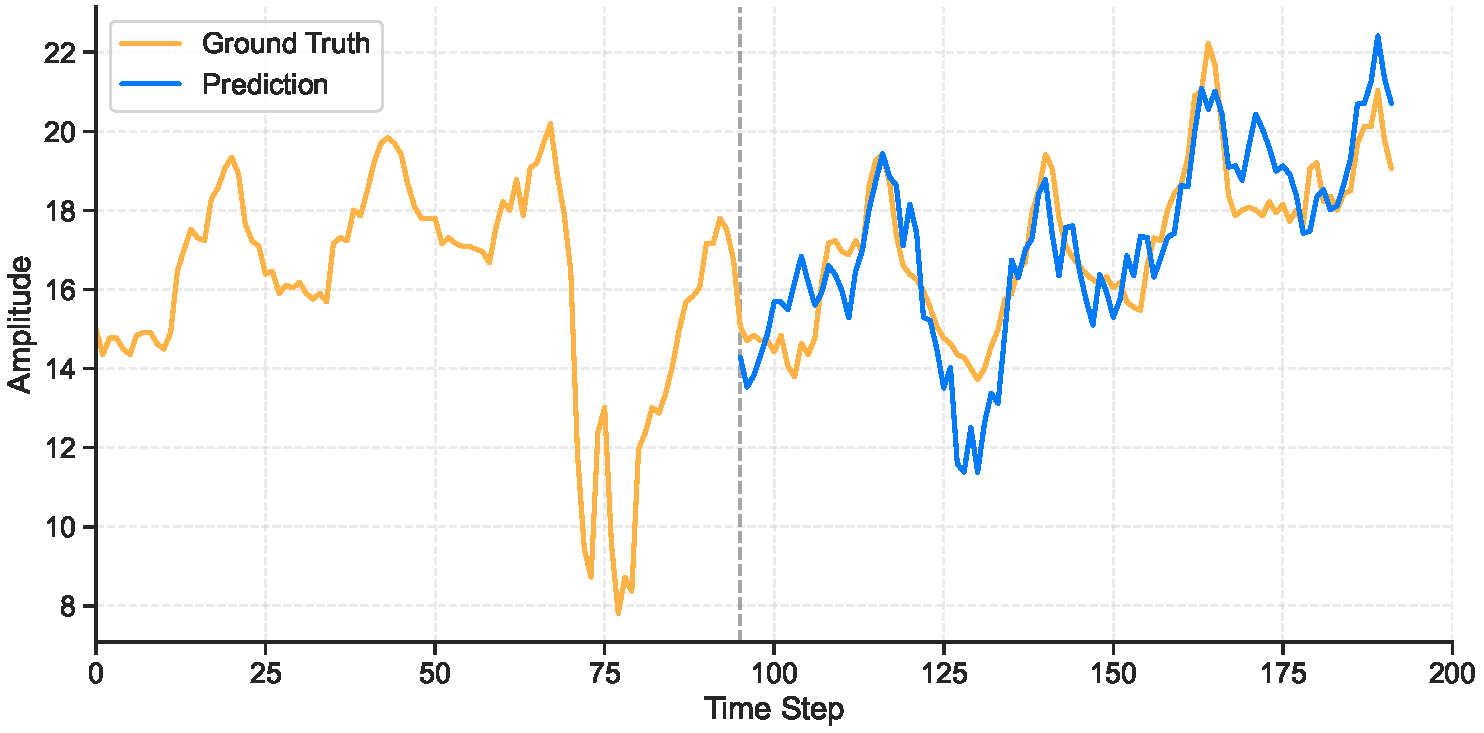
\includegraphics[width=\linewidth]{figures/showcase/ground_truth_plot_03_mse.pdf}\caption{Low prediction accuracy (high MSE).}\label{fig:showcase02-mse}\end{subfigure}%
\hfill%
\begin{subfigure}[t]{0.32\linewidth}\centering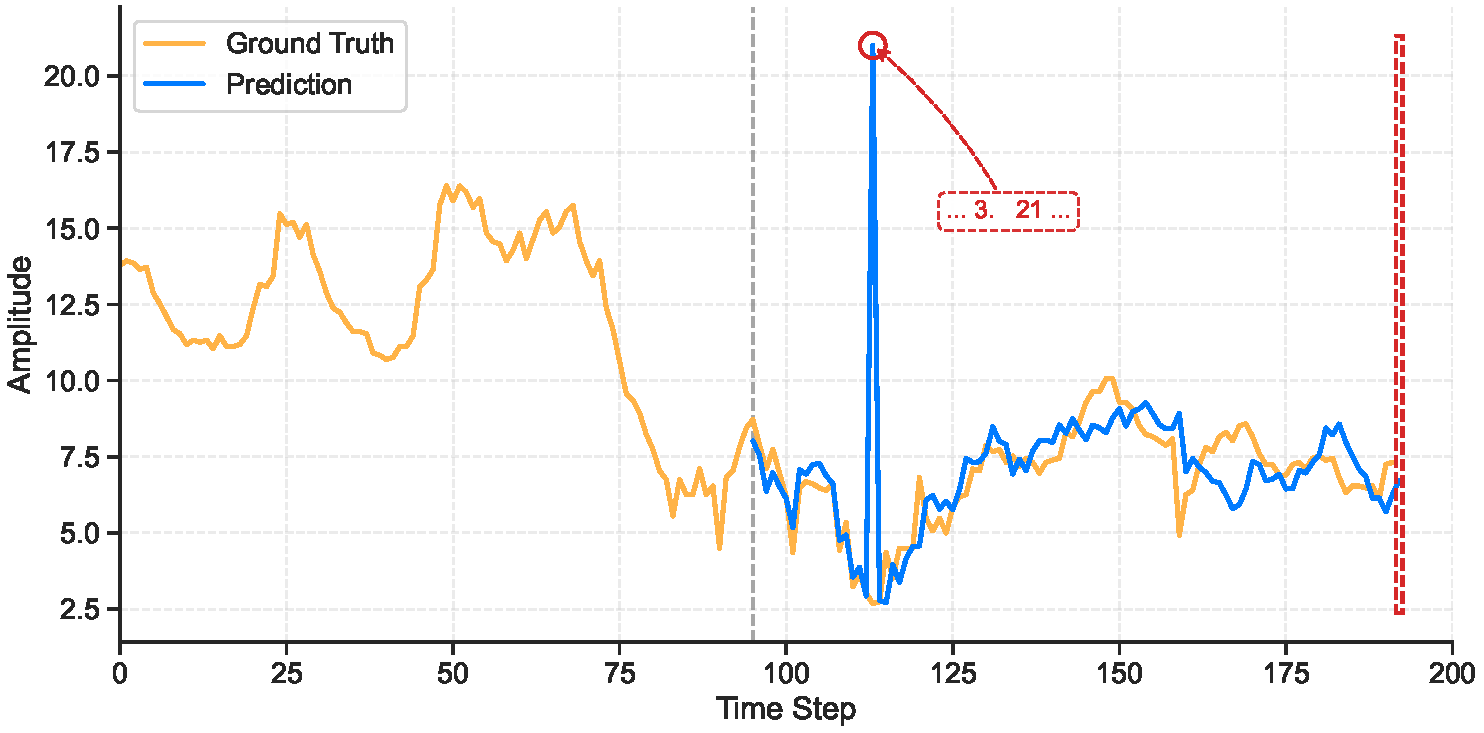
\includegraphics[width=\linewidth]{figures/showcase/ground_truth_plot_05_decimal.pdf}\caption{Formatting error causing abnormal spikes.}\label{fig:showcase03-fmt}\end{subfigure}%
\par\medskip
\begin{subfigure}[t]{0.32\linewidth}\centering
\includegraphics[width=\linewidth]{figures/showcase/ground_truth_plot_01.pdf}\caption{Correction of prediction length.}\label{fig:showcase01}\end{subfigure}%
\hfill%
\begin{subfigure}[t]{0.32\linewidth}\centering
\includegraphics[width=\linewidth]{figures/showcase/ground_truth_plot_03.pdf}\caption{Enhanced prediction precision.}\label{fig:showcase02}\end{subfigure}%
\hfill%
\begin{subfigure}[t]{0.32\linewidth}\centering
\includegraphics[width=\linewidth]{figures/showcase/ground_truth_plot_05.pdf}\caption{Rectification of output format and outliers.}\label{fig:showcase03}\end{subfigure}%

\caption{Showcase visualizations of input-96-predict-96 results on the ETTh1 dataset. The top row (a--c) displays the baseline performance of the STIT model, which exhibits limitations in sequence length, accuracy, and output formatting. The bottom row (d--f) shows the improvements achieved after applying the proposed RDFR framework. More showcases are provided in \shortautoref{appx:showcase_addition}.}\label{fig:showcases}\end{figure}


To intuitively understand how our proposed \textit{Temporal Refinement Reward System} in RDFR stage refines the model's behavior, we visualize a comparison between the STIT baseline and the final \method{} model in \shortautoref{fig:showcases}. This qualitative analysis targets three representative failure modes, validating the necessity of our composite reward system.

\textbf{Correction of Prediction Length}
As observed in \shortautoref{fig:showcase01-len}, the STIT model frequently suffers from "early stopping," failing to track the generation count and terminating the sequence before reaching the required horizon. This indicates a lack of internal counting logic. In contrast, \shortautoref{fig:showcase01} demonstrates the impact of the \textbf{Sequence Length Consistency Reward ($R_{len}$)}. By imposing a soft exponential length constraint, the RDFR stage forces the model to attend to the output length, ensuring the generated sequence perfectly matches the target horizon without truncation.

\textbf{Enhancement of Prediction Precision}
\shortautoref{fig:showcase02-mse} illustrates a case where the STIT model captures the general trend direction but fits loosely to the ground truth, exhibiting high variance and failing to capture local volatility. This corresponds to the limitations of token-level tuning in forecasting tasks. \shortautoref{fig:showcase02} showcases the refinement achieved via the \textbf{Prediction Accuracy Reward ($R_{acc}$)}. With its exponential scaling, $R_{acc}$ penalizes even minor deviations in the high-precision regime, driving the model to produce a curve that hugs the ground truth tightly and significantly reducing the MSE.

\textbf{Rectification of Formatting and Outliers}
Most critically, \shortautoref{fig:showcase03-fmt} reveals a severe "Integer Projection" hallucination where the STIT model fails to generate the decimal point (e.g., splitting a value like `3.21` into two tokens `3` and `21`). This formatting error inserts an extreme outlier into the time series and causes a phase shift in all subsequent data points. \shortautoref{fig:showcase03} confirms that the \textbf{Format Compliance Reward ($R_{fmt}$)} effectively eliminates this issue. By penalizing the model step-by-step for missing floating-point structures, the RDFR system enforces strict adherence to numerical syntax, restoring the smooth, continuous trajectory of the time series and preventing catastrophic outliers.

\subsection{Ablation and Sensitivity Analysis}
In this section, we perform comprehensive ablation studies to dissect the effectiveness of each component within the \method{} framework. Followed by \cite{jin2024timellm}, all experiments reported in this section are conducted on the \textbf{ETTh1} dataset with a fixed prediction horizon of $H=96$ unless otherwise explicitly stated.

\noindent\textbf{Component Analysis of the RDFR Framework.}\quad
To validate our design, we conducted an ablation study on the ETTh1 dataset. As shown in \shortautoref{tab:ablation_02}, while the off-the-shelf Qwen2.5-Instruct failed to generate valid outputs, the STIT model alone established a robust baseline with an MSE of \textbf{0.403}. This pivotal result demonstrates that complex pre-alignment modules are unnecessary; instruction tuning alone provides sufficient modality awareness for the LLM to function as a competent forecaster. Building on this foundation, the RDFR stage proved essential for precision. By imposing strict structural constraints and accuracy-driven rewards, the final RDTU framework further reduced the MSE to \textbf{0.351} with a \textbf{12.90\%} improvement over the STIT baseline, confirming that reinforcement learning effectively bridges the gap between basic instruction following and high-precision regression.

\input{tables/ablation02}

\begin{figure}[htbp]
    \centering

    \begin{subfigure}[t]{0.45\linewidth}
        \centering
        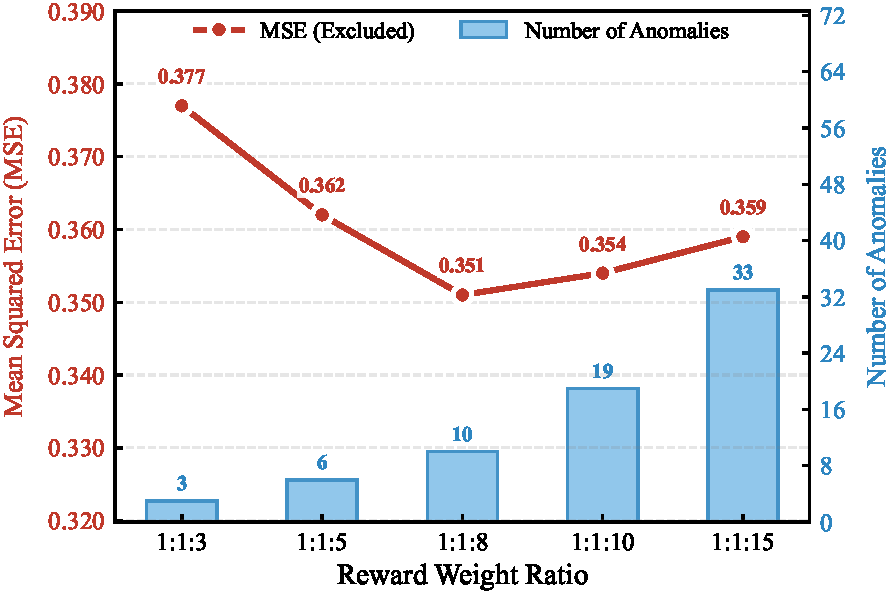
\includegraphics[width=\linewidth]{figures/ablation/ablation01.pdf}
        \caption{Impact of the reward weight ratio.}
        \label{fig:ablation_01}
    \end{subfigure}
    \hfill
    \begin{subfigure}[t]{0.52\linewidth}
        \centering
        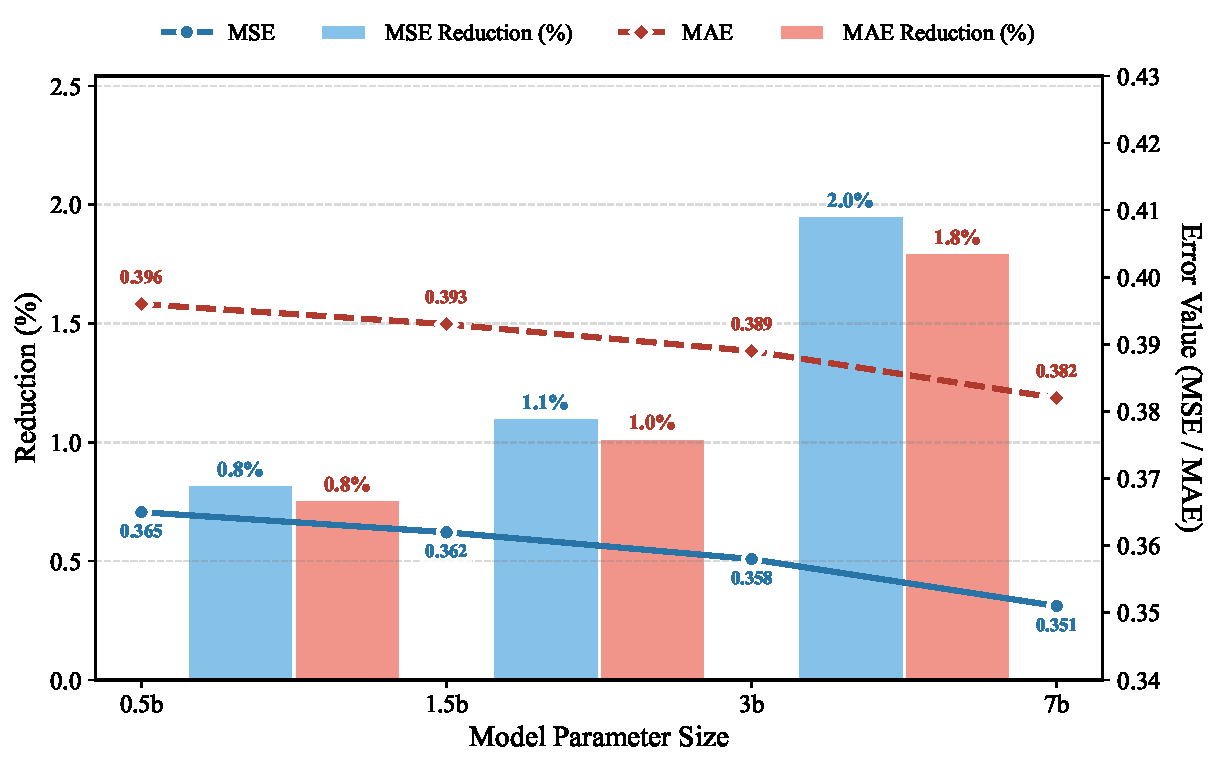
\includegraphics[width=\linewidth]{figures/ablation/ablation03_combined.pdf}
        \caption{Scaling laws on training efficiency and forecasting performance.}
        \label{fig:ablation_03}
    \end{subfigure}


    \caption{Ablation analysis of reward weighting and model scaling. Left: the red line represents the Mean Squared Error (MSE) on the excluded dataset, while the blue bars indicate the number of detected anomalies. Right: the line chart tracks MSE and MAE, showing that increased model capacity leads to consistent improvements in prediction accuracy.}
    \label{fig:ablation_combined}

\end{figure}


\noindent\textbf{Impact of Reward Weight Ratios.}\quad
We investigate the optimal balance between structural constraints and regression precision by varying the accuracy reward weight $\lambda_{acc}$ (fixing $\lambda_{len}:\lambda_{fmt}$ at $1:1$). Results on ETTh1 identify $\mathbf{1:1:8}$ as the optimal configuration, achieving the lowest MSE of \textbf{0.351}. Deviating from this equilibrium degrades performance via two distinct failure modes: low weights ($1:1:3$) result in under-optimization of numerical values (MSE 0.377), while excessive weights ($1:1:15$) induce "structural collapse." As shown in \shortautoref{fig:ablation_01}, pushing beyond the optimal threshold causes formatting anomalies to spike from 10 to 33, demonstrating that overpowering syntax constraints with accuracy objectives ultimately corrupts prediction validity.

\noindent\textbf{Impact of Model Scaling.}\quad
We evaluate the impact of model capacity across the Qwen2.5 family (0.5B, 1.5B, 3B, 7B). Results in \shortautoref{fig:ablation_03} reveal a robust scaling law: as parameter count increases, forecasting accuracy consistently improves, with MSE on ETTh1 monotonically decreasing from 0.365 (0.5B) to 0.351 (7B). This confirms that \textbf{RDTU} effectively harnesses the stronger reasoning capabilities of larger backbones to achieve finer precision.
